%% Results chapter
%% author Liu Peng

After designing and implementing the application. I conducted several
evaluation tests on the streaming performance. We had released the first
edition of the application in Google Play Store in Nov 2013. Since then, we had
been updating the application in order to improve its performance and enrich
its features. During the past year, we have collected a big amount of
useful data and interesting results.

This chapter presents the results of our evaluation. Section \ref{4_1} evaluates
the streaming performance of different streaming protocols. Section \ref{4_2}
presents the statistics from our users. Section \ref{4_3} provides a user study
and describes how we have improved the usability of our solution by utilizing
this study.
\subsection{Evaluation of streaming performance\label{4_1}}
In terms of streaming, our solution includes two major streaming components. It
would be helpful to study and compare which streaming protocol has the better
performance while streaming multimedia contents in different network conditions.
The two major streaming technologies we used in our solution are HTTP streaming
and RAOP streaming, respectively.

Hypertext Transfer Protocol (HTTP) \cite{http_rfc} is the protocol used to
deliver web pages and images across the World Wide Web. HTTP is a most widely adopted, open
standard and the most ubiquitous method of content delivery on the Internet.
HTTP objects can be delivered by a variety of web servers, including
commercially used servers and open source
servers\footnote{\url{http://blog.eduguru.in/http-versus-rtmp-which-way-to-go-and-why/}}.
Both DLNA and Chromecast utilize HTTP to realize their streaming functionality.

Unlike HTTP, another popular protocol, the Real Time Streaming Protocol (RTSP)
\cite{rtsp_rfc} is a network control protocol used in entertainment and
communications systems to control media streaming servers. RTSP is used to establish and control media
sessions between two points, usually the server and player client. Clients of
media servers issue VCR-like commands, such as PLAY and PAUSE, to facilitate
real-time control of playback of media files from the
server\footnote{\url{http://blog.eduguru.in/http-versus-rtmp-which-way-to-go-and-why/}}.
The RAOP protocol, which is virtually another version of RTSP, is used by AirPlay, for
the streaming of iTunes music.

This section presents the evaluation of HTTP and RTSP streaming servers and
compares the streaming performance in different network conditions. Since we
have both protocols implemented in our application, we could compare the
performance by streaming the same content to two receivers using the two
different protocols. Typically, DLNA music streaming uses HTTP protocol and
AirPlay music streaming uses ROAP protocol. After the experimental setup
described in Section \ref{3_7_1}, we conducted three different experiments.
Section \ref{4_1_1} compares the streaming traffic of DLNA and AirPlay
standards. Section \ref{4_1_2} compares the streaming performance of DLNA and
AirPlay in limited bandwidth situation. Section \ref{4_1_3} presents a
similar comparison but under high packet loss scenarios.
\subsubsection{Comparison of AirPlay and DLNA traffic\label{4_1_1}}
After the initial experimental setup described in Section \ref{3_7_1}, we
selected an mp3 music file and streamed it to both an AirPlay receiver
and a DLNA receiver, and we used Wireshark running on the laptop to capture the
packets in the network.

After the experiment environment is set up, a series of tests is conducted and
the result is presented in Figure \ref{airplay_vs_dlna_traffic}.

According to the result, the stream traffics of AirPlay and DLNA streaming are
very different. Figure \ref{airplay_vs_dlna_traffic_a} shows the scenario of
AirPlay music streaming, x-axis is the duration of the stream since the
beginning of the music; y-axis is the total traffic in bytes accumulated since
the beginning of the stream. There are two lines which represents the total
data and non-retransmitted data separately. According to this figure, the
traffic growth of AirPlay streaming is nearly linear, only two slow-downs
occurred at 1:30 and 2:00 due to network condition. This is because ROAP is a
push like process and content can be streamed in real time.

In contrast, Figure \ref{airplay_vs_dlna_traffic_b} shows that in DLNA
streaming, there are clearly two phases in the traffic graph. During the first
20 seconds, the amount of traffic grows rapidly. After that, the traffic growth slowed down and
keeps the same increase rate till the end of the stream. The reason behind it
is that HTTP streaming is a pull like process, the server can actively fetch
content from the media server and the content can be buffered up since the
beginning of the playback, with the best effort of the network. Therefore,
there is a short download period at the beginning of the DLNA streaming graph.
After all the content is buffered already, the traffic growth is the result of
constantly updating of playback status.
\begin{figure}[hb]
\subfigure[AirPlay\label{airplay_vs_dlna_traffic_a}]{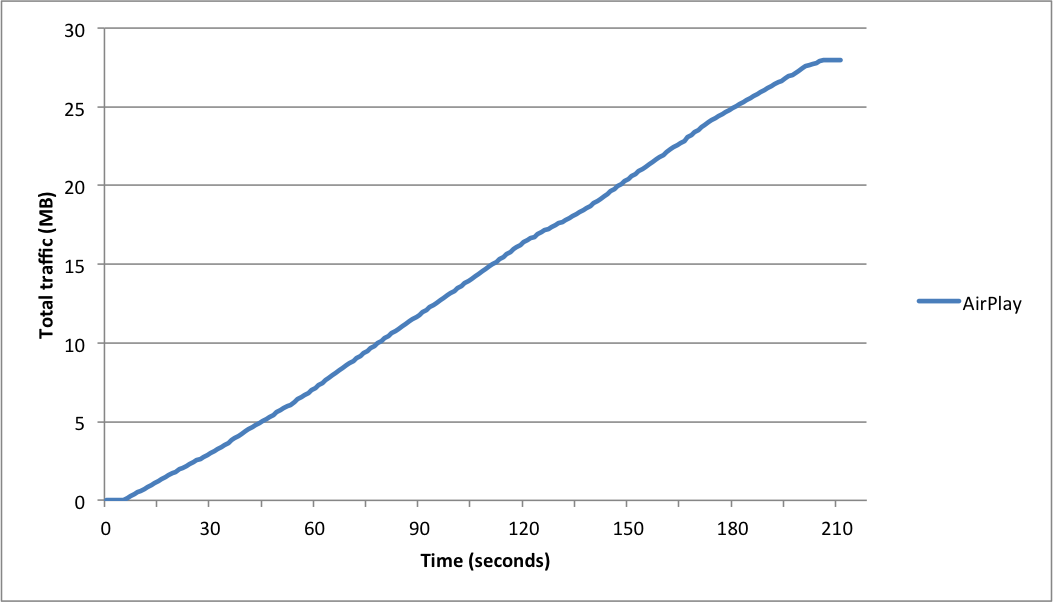
\includegraphics[width=0.9\columnwidth]{charts/accu_airplay}}
\subfigure[DLNA\label{airplay_vs_dlna_traffic_b}]{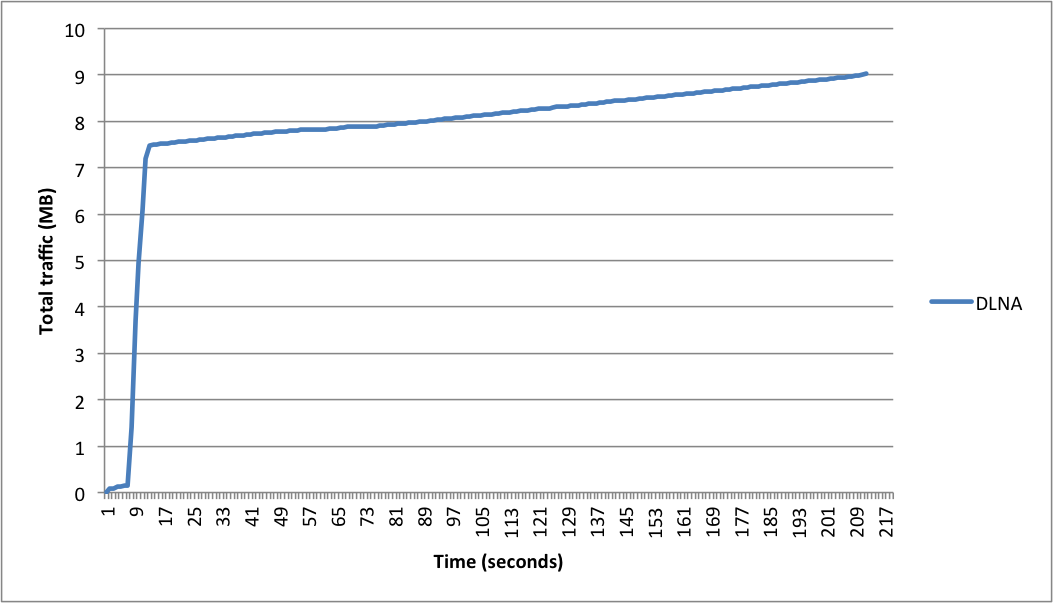
\includegraphics[width=0.9\columnwidth]{charts/accu_dlna}}
\caption{AirPlay vs DLNA streaming traffic
comparison \label{airplay_vs_dlna_traffic}}
\end{figure}
\clearpage

In addition, as shown in Figures \ref{airplay_vs_dlna_traffic_a} and
\ref{airplay_vs_dlna_traffic_b}, the total bytes of AirPlay streaming is 27
megabytes while the total bytes of DLNA streaming is 9 megabytes. The
AirPlay streaming consumes two times more traffic than the DLNA streaming. This
is because AirPlay uses Apple Lossless Audio Codec (ALAC) format for music
streaming, as discussed in \ref{2_3_3_4}. Since ALAC is a lossless format, the
transcoding from the MP3 format to the ALAC format actually decompresses the
data, which increases the total size of media file significantly. This huge
difference of total traffic makes the AirPlay music streaming consume
significantly more energy than the DLNA streaming.

This comparison describes the different characteristics of HTTP streaming and
RAOP streaming. These differences could result in different performance and
user experience. In the following sections, we will identify these differences
by changing the network conditions. And finally we could draw the conclusion
which protocol is more suitable for multimedia home networking.
\subsubsection{Performance under limited bandwidth\label{4_1_2}}
During this experiment, we reused the same setup mentioned in Section
\ref{3_7_1}, in addition, different bandwidth limitations are introduced. We
evaluate the performance of the two streaming solutions under limited
bandwidth. The bandwidth is limited to 500 kbps, 700 kbps and 1000 kbps
respectively in three rounds of tests. During each round of the test, the same
mp3 music is streamed to XBMC receiver using the DLNA standard and the AirPlay
standard. Figures \ref{all_traffic_bw} and \ref{all_traffic_bw_1} show the
result of AirPlay and DLNA streaming.

DLNA graph of Figure \ref{all_traffic_bw_a} shows that when there is no limit
in bandwidth, there is a 20-second traffic burst during the initial phase of the
streaming, which means the loading speed is the fastest and most of the content
is already buffered in the first 20 seconds. DLNA graph in Figure
\ref{all_traffic_bw_b} shows the traffic graph when bandwidth is limited to
500kbps, the initial downloading phase takes around 230 seconds, which is ten
times more than the DLNA graph in Figure \ref{all_traffic_bw_a}. The bandwidth
limit influences the buffer time of DLNA streaming.

Figure \ref{all_traffic_bw_1_a} shows the total traffic graph when the
bandwidth is limited to 700kbps and Figure \ref{all_traffic_bw_1_b} shows the
traffic graph when the bandwidth is limited to 1000kbps. According to the
Figure \ref{all_traffic_bw_b}, \ref{all_traffic_bw_1_a} and
\ref{all_traffic_bw_1_b}, in terms of DLNA streaming, the initial loading speed
is dependent on the network bandwidth. When the network bandwidth is
limited, as the bandwidth of network increases, the initial loading speed would
also increase. This proves that in DLNA streaming, most of the content is fully
downloaded in the initial phase of streaming, because HTTP streaming is used in
this case. The quality of steaming can be guaranteed when the initial buffering
is finished. The receiver will take the buffered content and play locally.

In contrast, according to the AirPlay graphs shown in Figure
\ref{all_traffic_bw_a}, \ref{all_traffic_bw_b}, \ref{all_traffic_bw_1_a}, and
\ref{all_traffic_bw_1_a}, the traffic graph of AirPlay didn't change much
when the bandwidth is changed. This is because AirPlay music streaming is based
on ROAP, which is a RTP-like protocol. The transport layer protocol used is
UDP, thus not all packets are successfully delivered to the receiver. The UDP
based delivery only provides a best-effort transmission. In addition, RAOP
doesn't include the RTSP feedback functionality, which can be used to adaptively
adjust the streaming quality according to the network condition. The sound quality can not be
guaranteed because there is no buffer or retransmission mechanism on the
receiver side and the transmission is almost real-time. Given this reason, when
the bandwidth is limited to 500 kbps, the AirPlay playback is heavily
interrupted. All music information is lost since too many packets are lost
during the transmission. When the bandwidth is increased to 700 kbps, the
AirPlay playback still can not work properly. The playback is choppy and noisy.
After the bandwidth is increased to 1000 kbps, the music can then work smoothly
and no noticeable noise can be heard.

When comparing the difference of the amount of transferred bytes, Figure
\ref{all_traffic_bw_b} shows that AirPlay streaming generates more traffic than
DLNA streaming. This is due to the fact that in the case of AirPlay music
streaming, MP3 media is transcoded to ALAC format, which increased the
total amount of data to transfer. This difference also affects the energy
consumption significantly.

Another thing worth mentioning is that in the experiment, the same mp3 music is
used in both tests. But obviously the playback quality of DLNA is better than
the playback using AirPlay. For instance, when the bandwidth is limited to 500
kbps, AirPlay streaming is basically not usable any more, while DLNA streaming
is still working properly. The reason behind this is that in the case of DLNA
streaming, the original mp3 music is directly streamed to receiver, while in
the case of AirPlay music streaming, the same mp3 music is firstly decoded to
PCM format and then encoded to Apple Lossless format. Since mp3 is a compressed
media format while Apple Lossless format is an uncompressed media format, the
bandwidth required by DLNA streaming is considerably smaller than AirPlay
streaming.

As a conclusion, in the scenario of limited bandwidth, DLNA has the advantage
of sound quality compared to AirPlay standard. The buffer system, benefited
from HTTP streaming mechanism, gives DLNA a more reliable data flow. While
AirPlay streaming suffered from the packet loss of UDP and the sound quality is
heavily affected. Generally speaking, DLNA is more tolerant than AirPlay
streaming in the case of limited bandwidth. 
\begin{figure}[hb]%[!t]%[hb][!b]
\subfigure[No
limit\label{all_traffic_bw_a}]{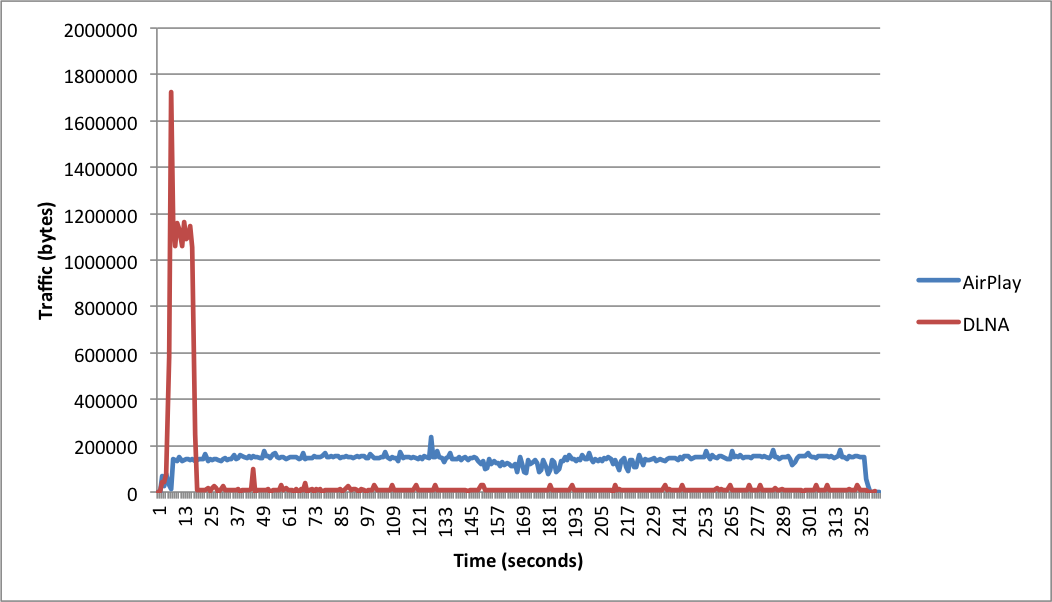
\includegraphics[width=1\columnwidth]{charts/bytes_nolimit}}
\subfigure[500kbps\label{all_traffic_bw_b}]{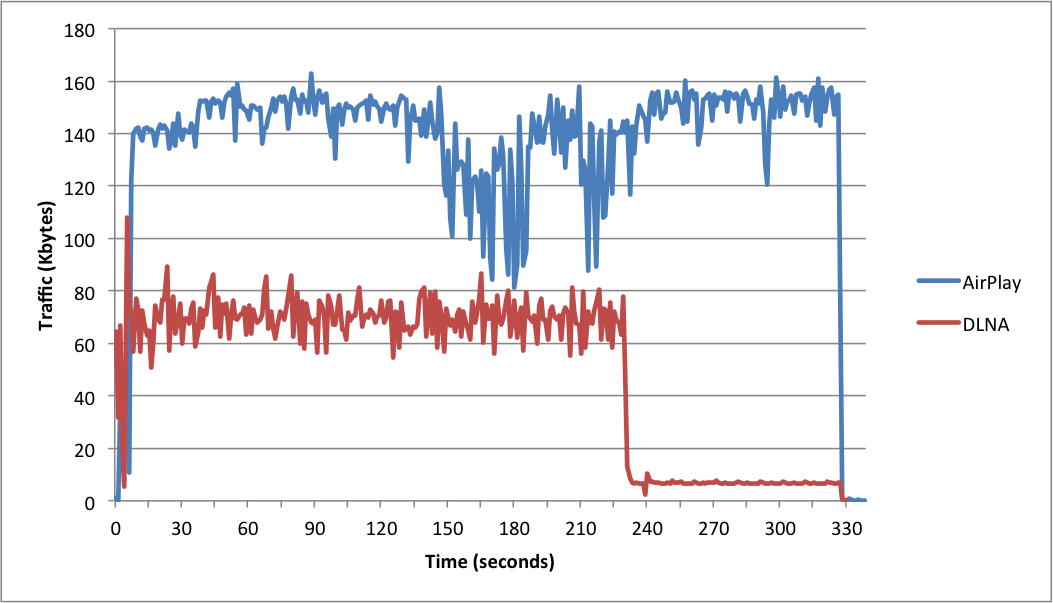
\includegraphics[width=1\columnwidth]{charts/bytes_500k}}
\caption{AirPlay and DLNA traffic in bandwidth constrained
situation\label{all_traffic_bw}}
\end{figure}
\begin{figure}[hb]%[!t]%[hb][!b]
\subfigure[700kbps\label{all_traffic_bw_1_a}]{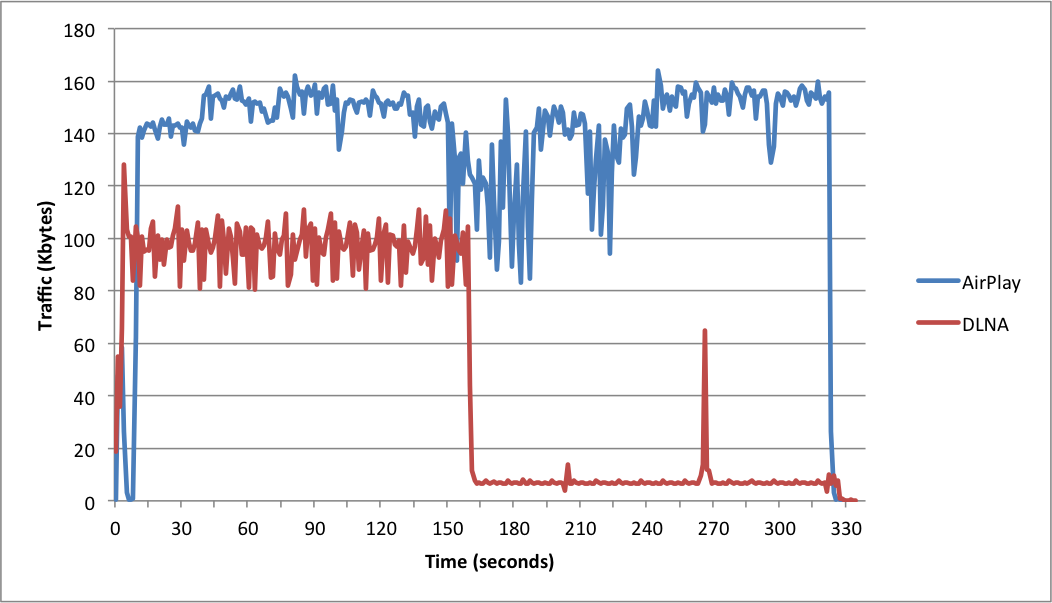
\includegraphics[width=1\columnwidth]{charts/bytes_700k}}
\subfigure[1000kbps\label{all_traffic_bw_1_b}]{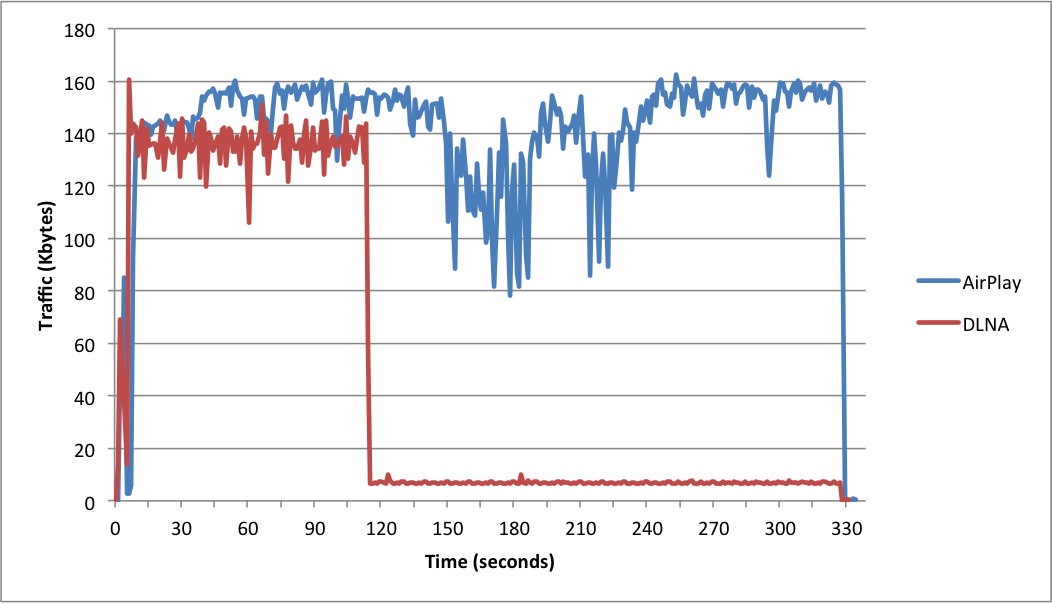
\includegraphics[width=1\columnwidth]{charts/bytes_1000k}}
\caption{AirPlay and DLNA traffic in
bandwidth constrained situation\label{all_traffic_bw_1}}
\end{figure}
\clearpage
\subsubsection{Influence of packet loss\label{4_1_3}}
After the bandwidth test, we then simulated packet loss on the receiver side and
conducted the same test for DLNA and AirPlay streaming with the same setup
described in \ref{3_7_1}. 5\%, 10\% and 15\% packet loss are introduced to test
both DLNA and AirPlay streaming. Figure \ref{dlna_pl} and \ref{dlna_pl_1} show
the result of DLNA streaming. Figure \ref{all_pl} and \ref{all_pl_1} show the
overall traffic graph of AirPlay and DLNA streaming in four different packet
loss situations.

According to DLNA graph in Figure \ref{dlna_pl_a}, when there is no packet
loss, very little retransmission data is seen in the graph and the initial
download phase takes only 17 seconds to finish. DLNA graphs in Figure
\ref{dlna_pl_b} and \ref{dlna_pl_1_a} shows that when the packet loss ratio is
increased from 5\% to 10\%, the portion of retransmitted data is getting larger
and larger, and according to DLNA graphs in Figure \ref{all_pl_b} and
\ref{all_pl_1_a}, the download time increased from 25 seconds to 57 seconds.
However, there is no noticeable loss of sound quality since the whole music is
buffered before the end of the song. As DLNA graph shown in Figure
\ref{dlna_pl_1_b}, when the packet loss ratio is increased to 15\%, significant
amount of retransmission can be found in the graph, and DLNA graph in Figure
\ref{all_pl_1_b} shows the buffering traffic becomes very choppy, the music
is not fully buffered even after the time duration of the music is reached, and
the streaming stopped for buffering three times during one song's playback. In the
case of DLNA streaming, packet loss is a key impediment. When packet loss rate
climbs to a certain point, for instance 15\% in this test, the streaming
becomes unusable.

The same packet loss tests on AirPlay streaming was also conducted and the
results are shown in AirPlay graphs in Figure \ref{all_pl} and \ref{all_pl_1}.
According to Figure \ref{all_pl_a}, \ref{all_pl_b}, \ref{all_pl_1_a}, and
\ref{all_pl_1_b}, in the case of AirPlay streaming, the traffic graph is
relatively stable, and does not vary when packet loss is changed, this is
because UDP is used during the AirPlay playback, the ROAP server embedded in
Streambels keeps sending data to the receiver using UDP regardless of the
packet loss. On the receiver side, the player tries its best to decode the
broken data. There is no mechanism for acknowledgement or retransmission.
Surprisingly, the sound quality is much better compared with DLNA streaming.
The reason behind is that retransmission of TCP consumes more and more
bandwidth in the case of DLNA streaming, in the same situation.
AirPlay streaming instead tries to deliver all contents with its best effort,
without creating extra demand for retransmission.

In a nutshell, in the case of packet loss, AirPlay is more tolerant to packet loss than DLNA.
\begin{figure}[hb]
\subfigure[No
limit\label{dlna_pl_a}]{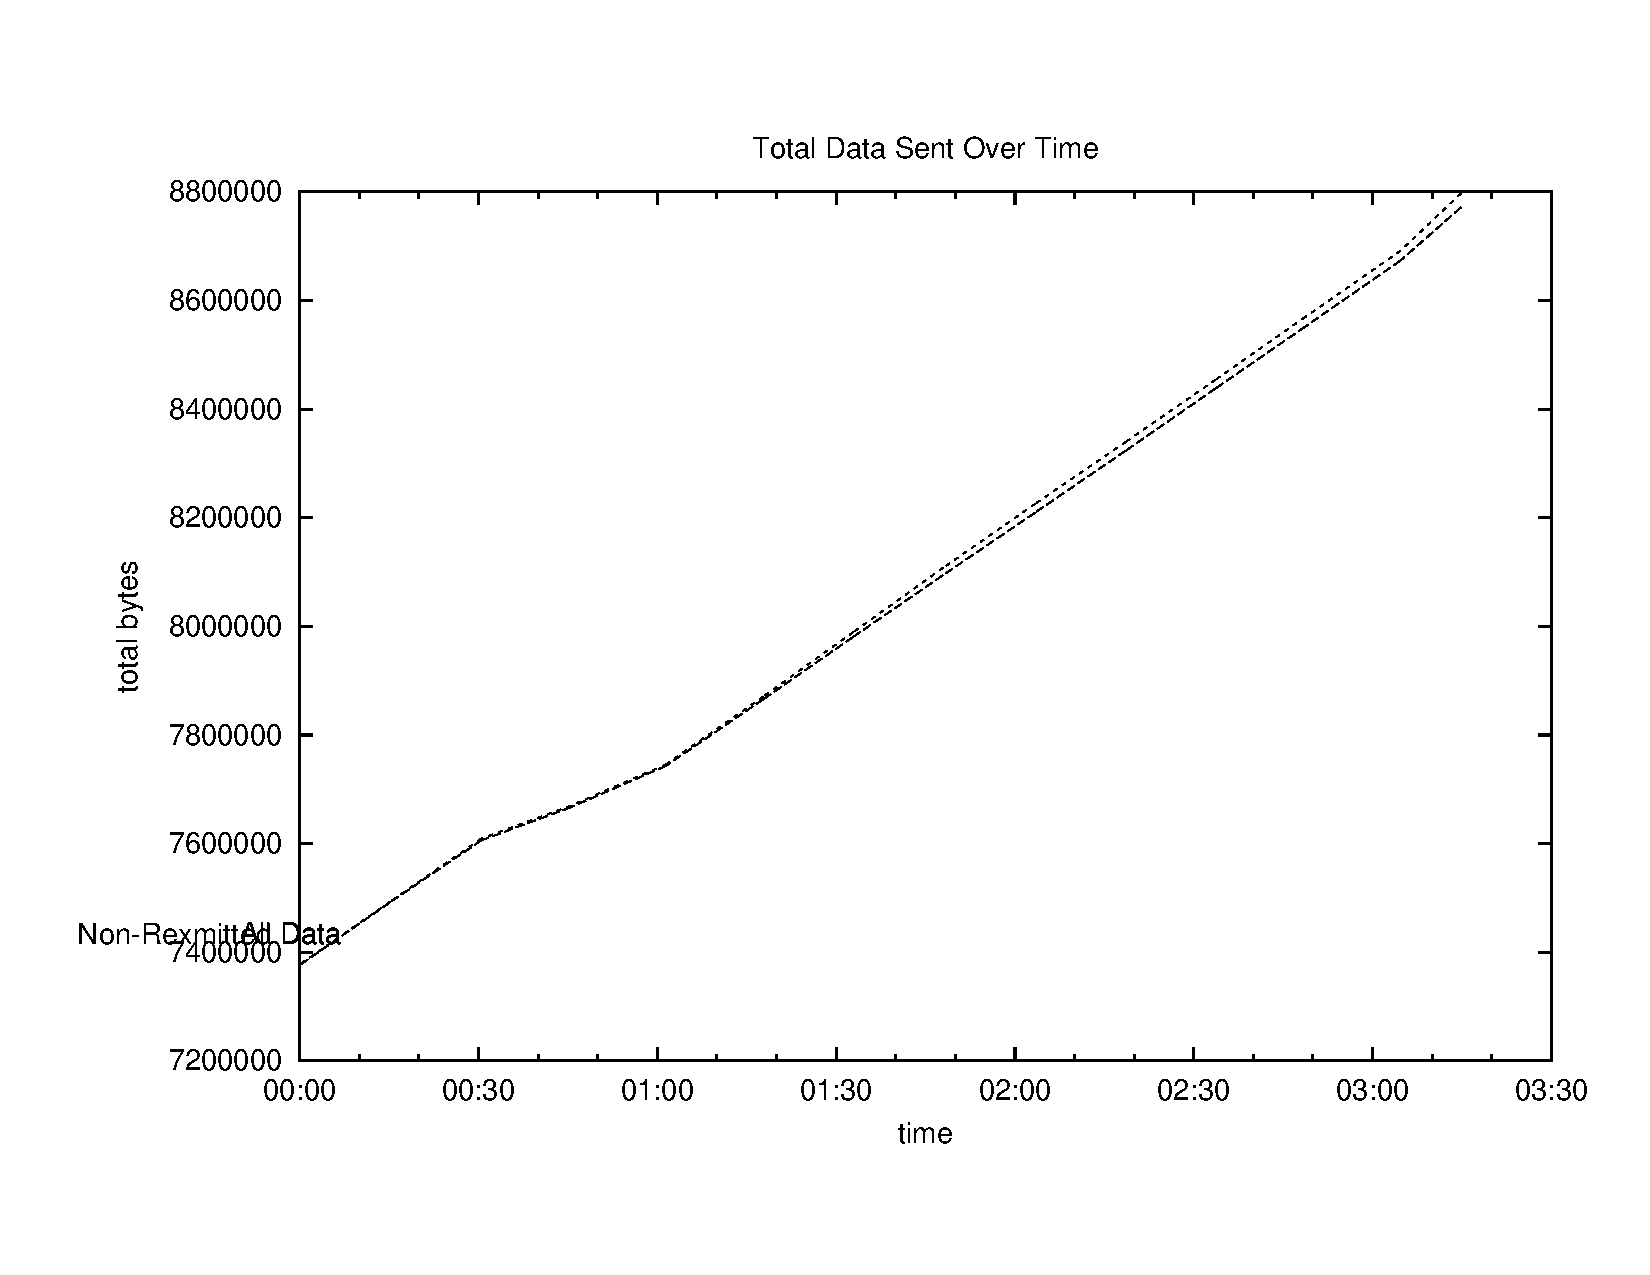
\includegraphics[width=0.9\columnwidth]{charts/dlna_traffic_data}}
\subfigure[5
percent
loss\label{dlna_pl_b}]{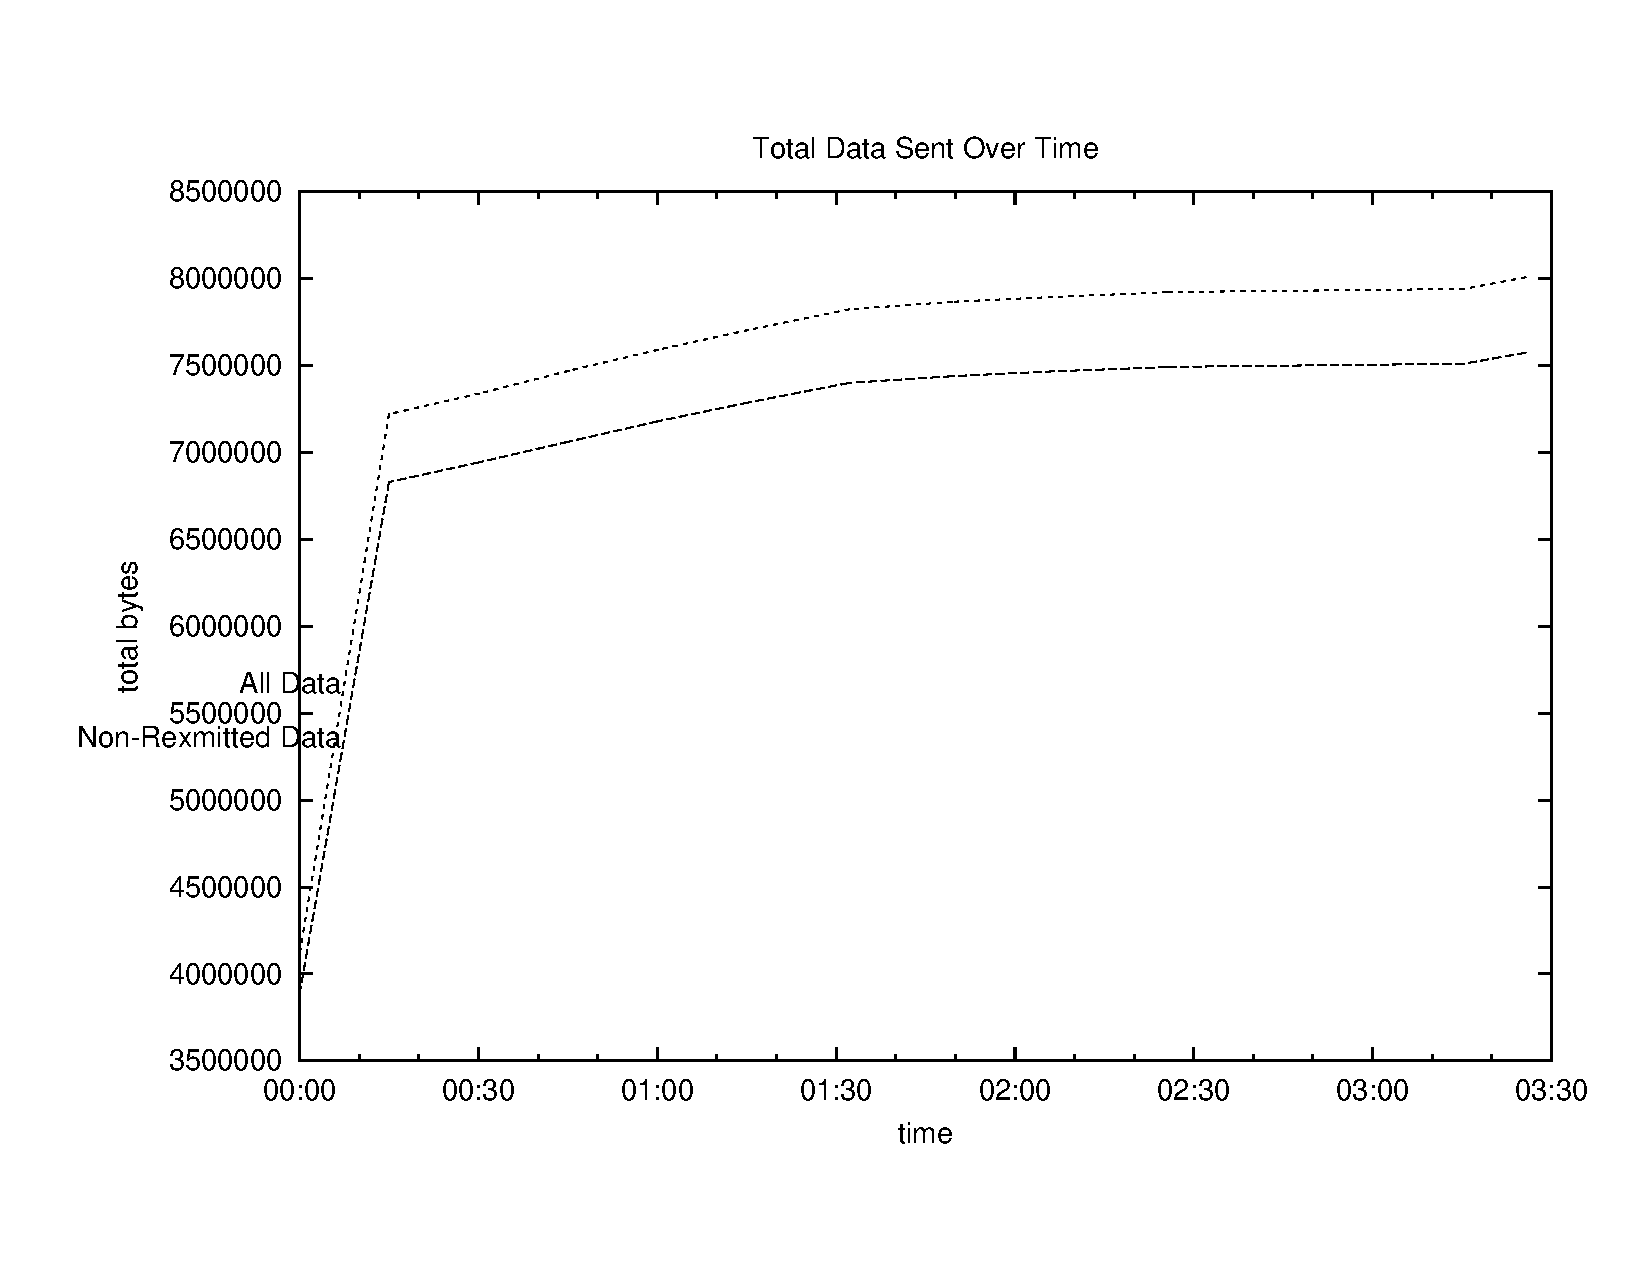
\includegraphics[width=0.9\columnwidth]{charts/dlna_traffic_5loss_data}}
\caption{DLNA accumulated traffic in terms of packet loss
\label{dlna_pl}}
\end{figure}

\begin{figure}[hb]
\subfigure[10
percent
loss\label{dlna_pl_1_a}]{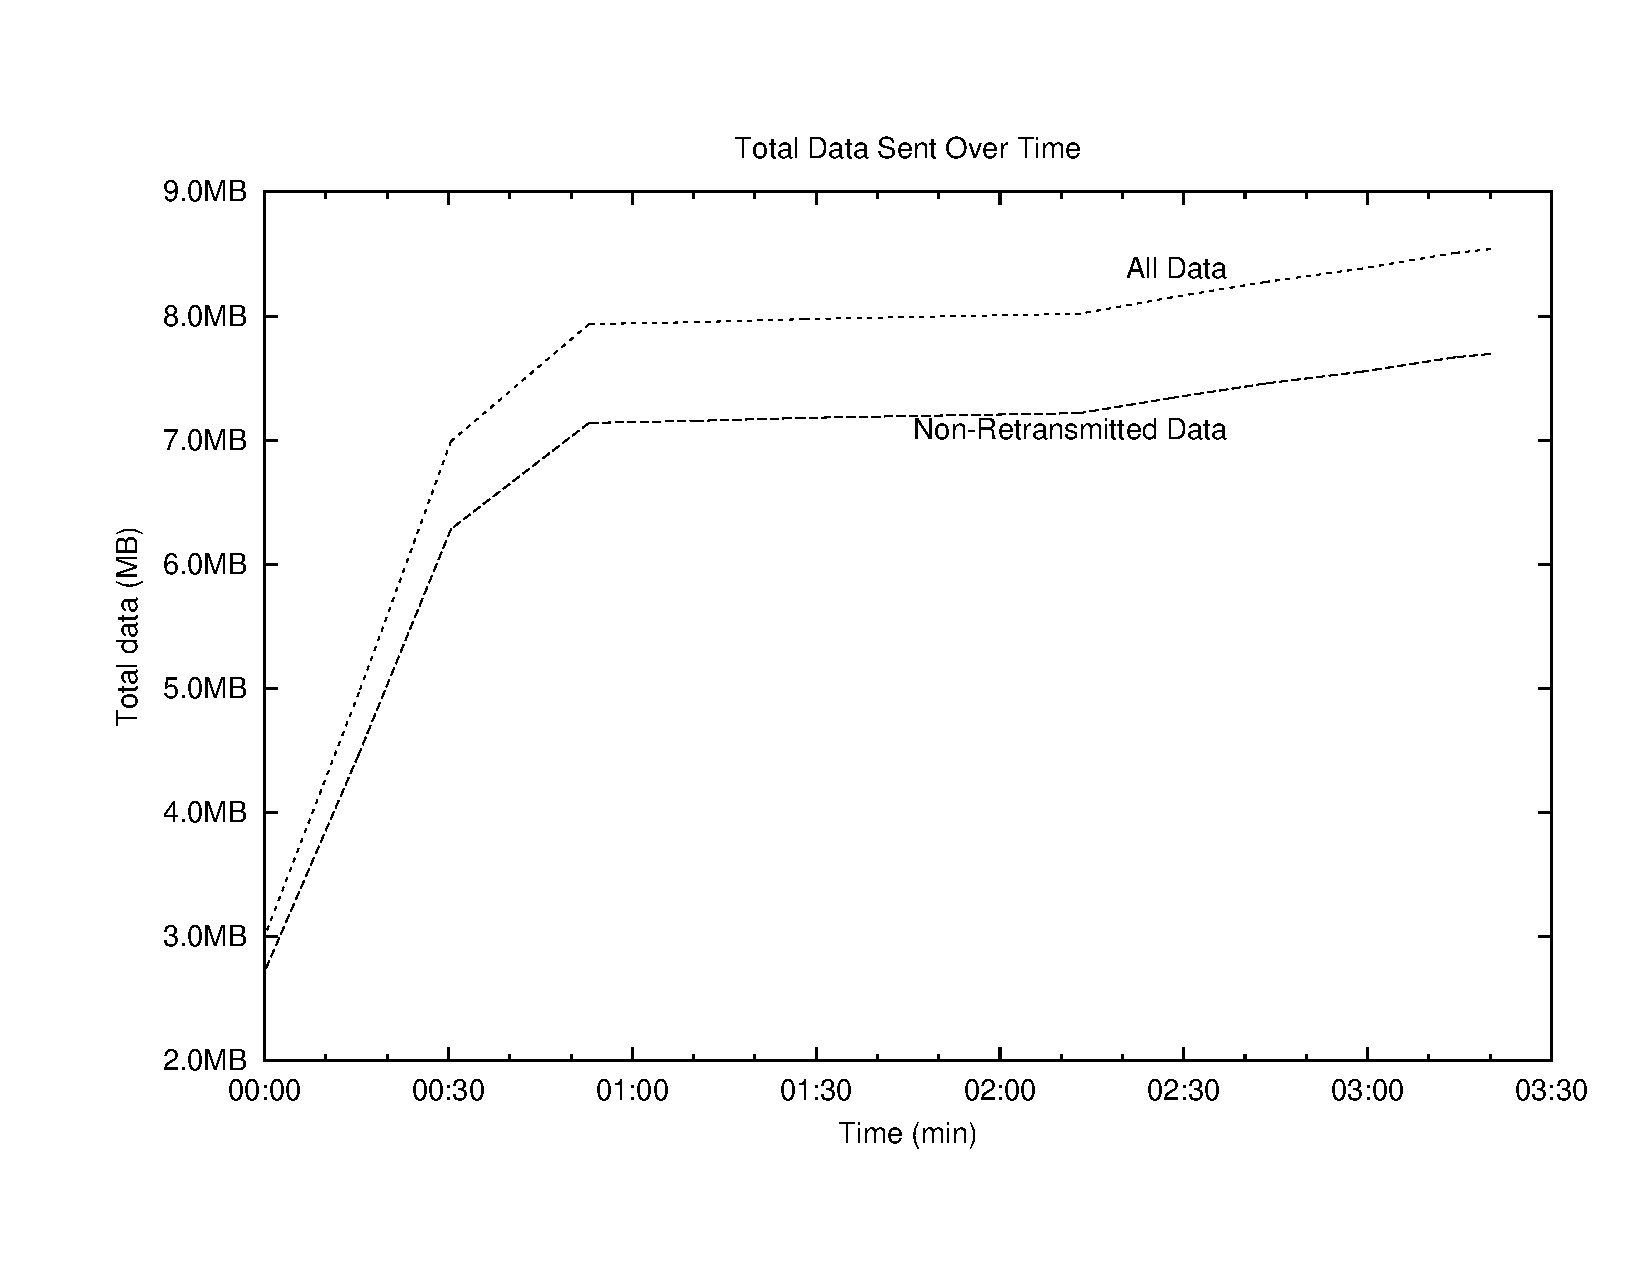
\includegraphics[width=0.9\columnwidth]{charts/dlna_traffic_10loss_data}}
\subfigure[15 percent
loss\label{dlna_pl_1_b}]{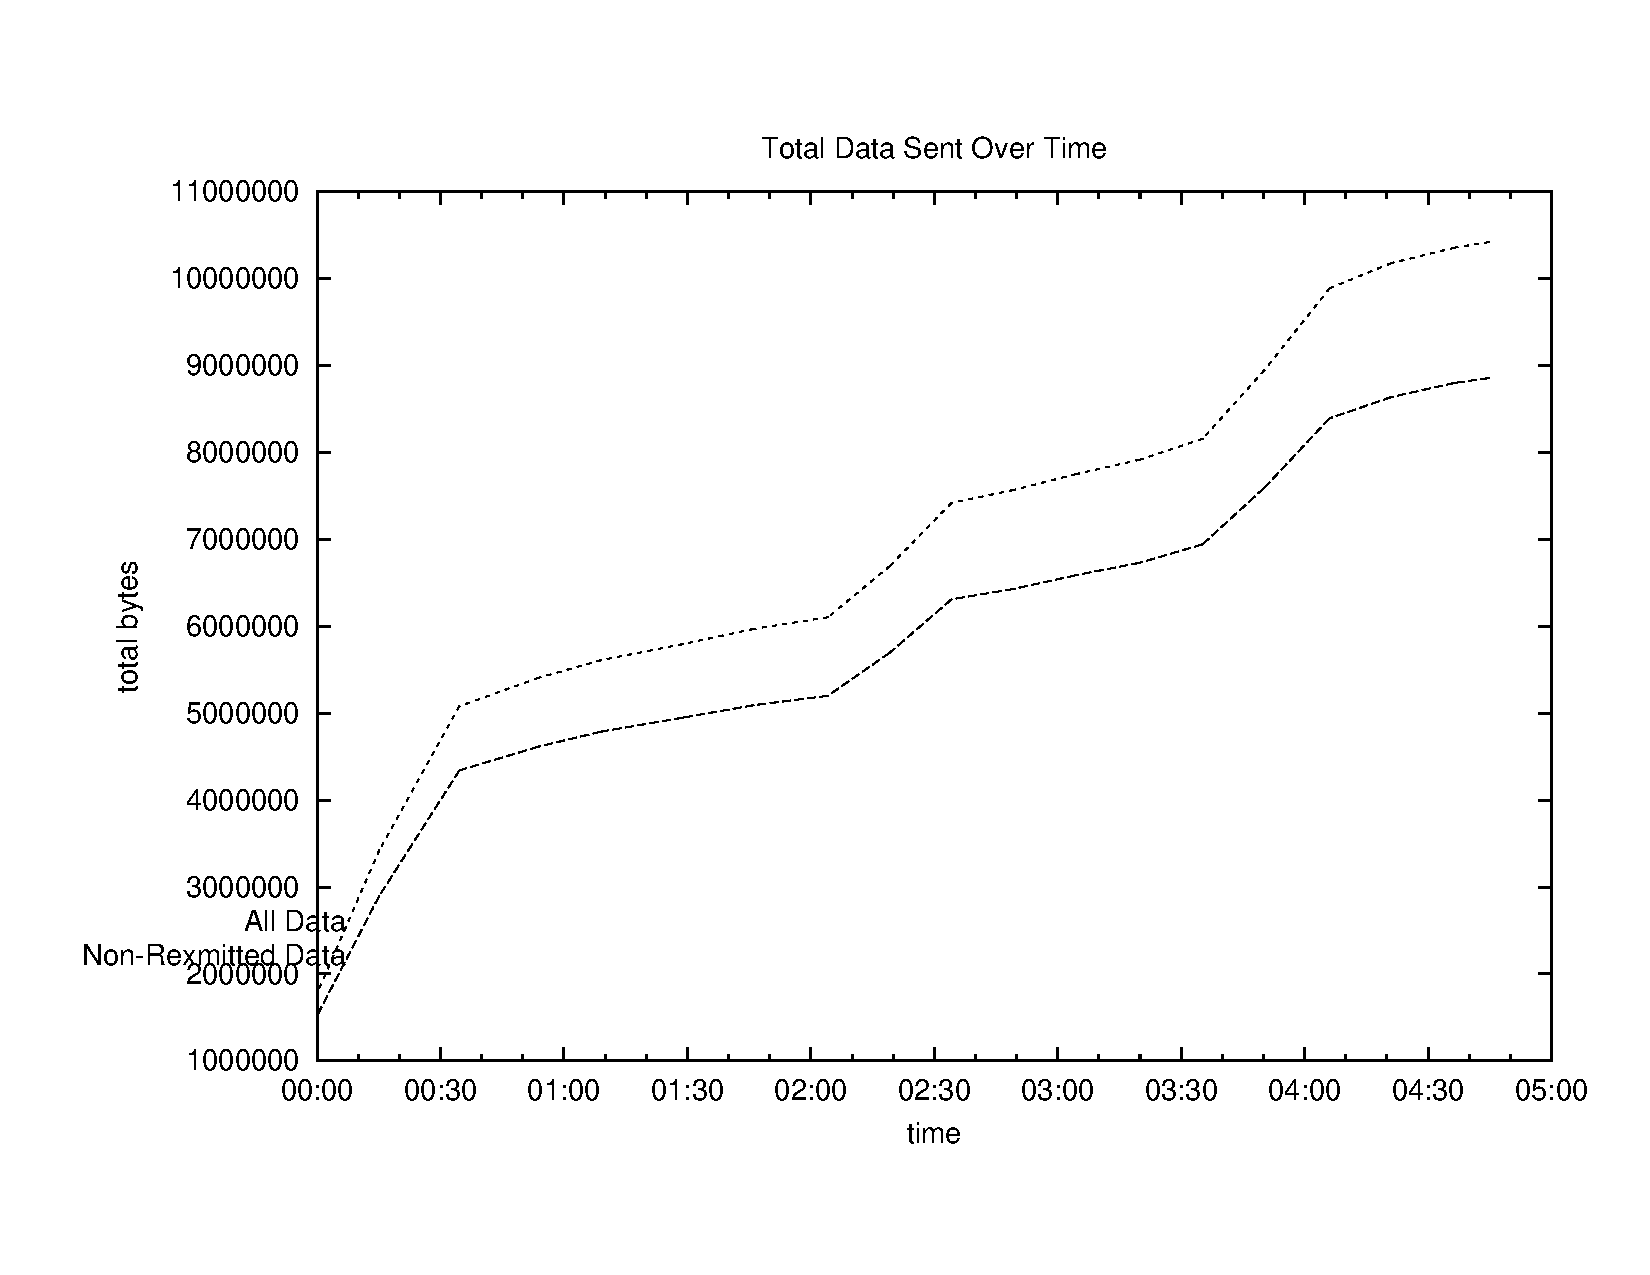
\includegraphics[width=0.9\columnwidth]{charts/dlna_traffic_15loss_data}}
\caption{DLNA accumulated traffic in terms of packet loss \label{dlna_pl_1}}
\end{figure}

\begin{figure}[hb]
\subfigure[No
limit\label{all_pl_a}]{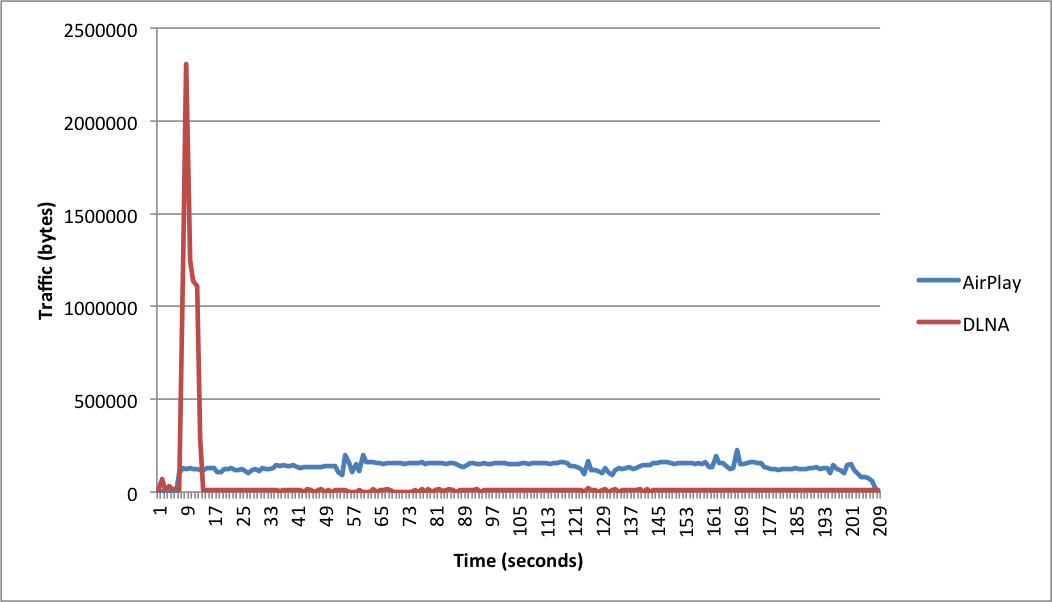
\includegraphics[width=1\columnwidth]{charts/packetloss_nolimit}}
\subfigure[5
percent
loss\label{all_pl_b}]{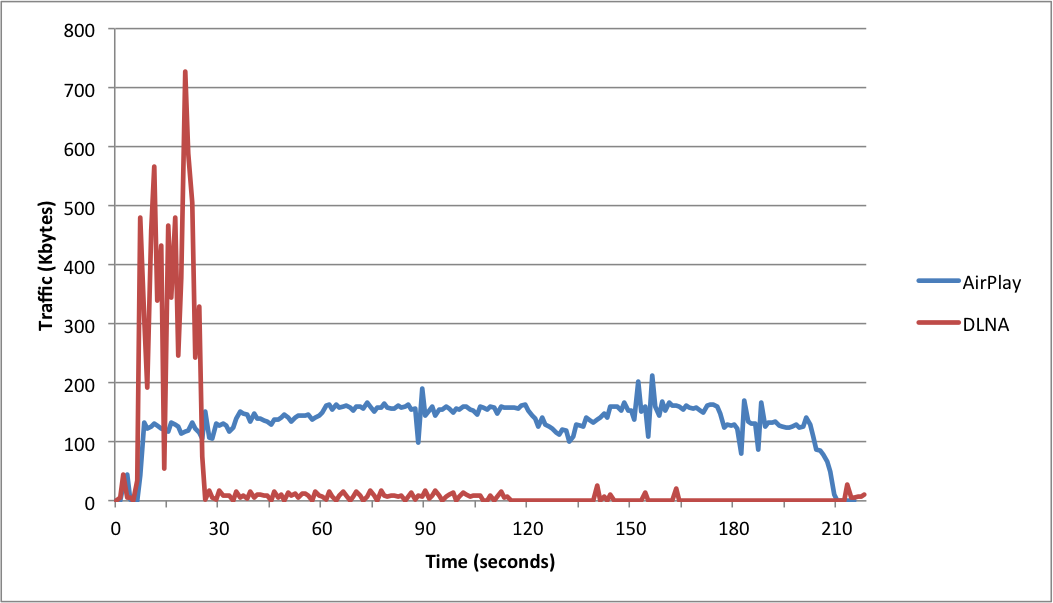
\includegraphics[width=1\columnwidth]{charts/packetloss_5percent}}
\caption{AirPlay and DLNA traffic graph in terms of packet loss \label{all_pl}}
\end{figure}

\begin{figure}[hb]
\subfigure[10
percent
loss\label{all_pl_1_a}]{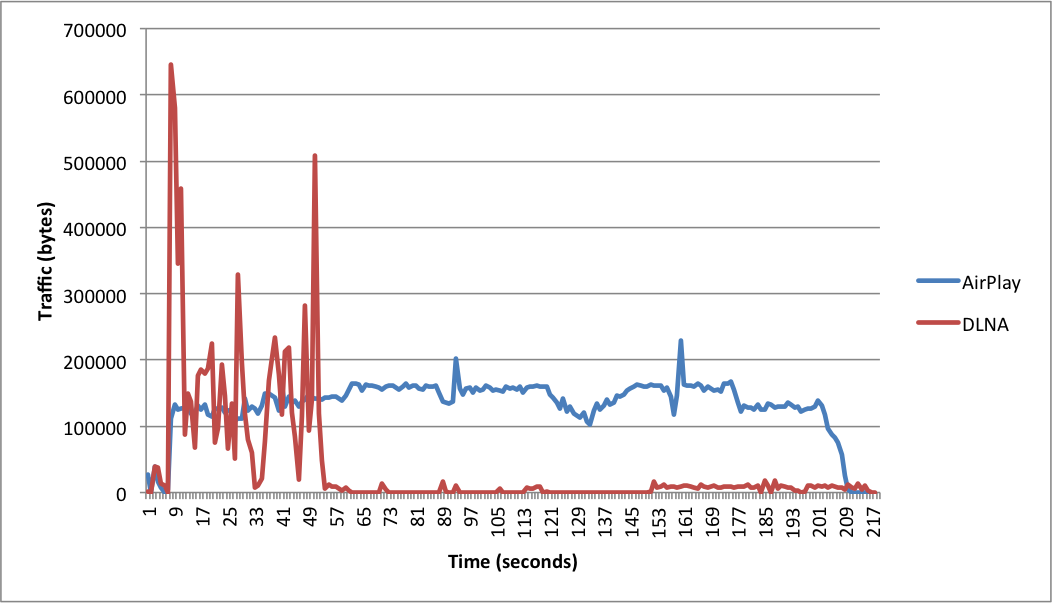
\includegraphics[width=1\columnwidth]{charts/packetloss_10percent}}
\subfigure[15 percent
loss\label{all_pl_1_b}]{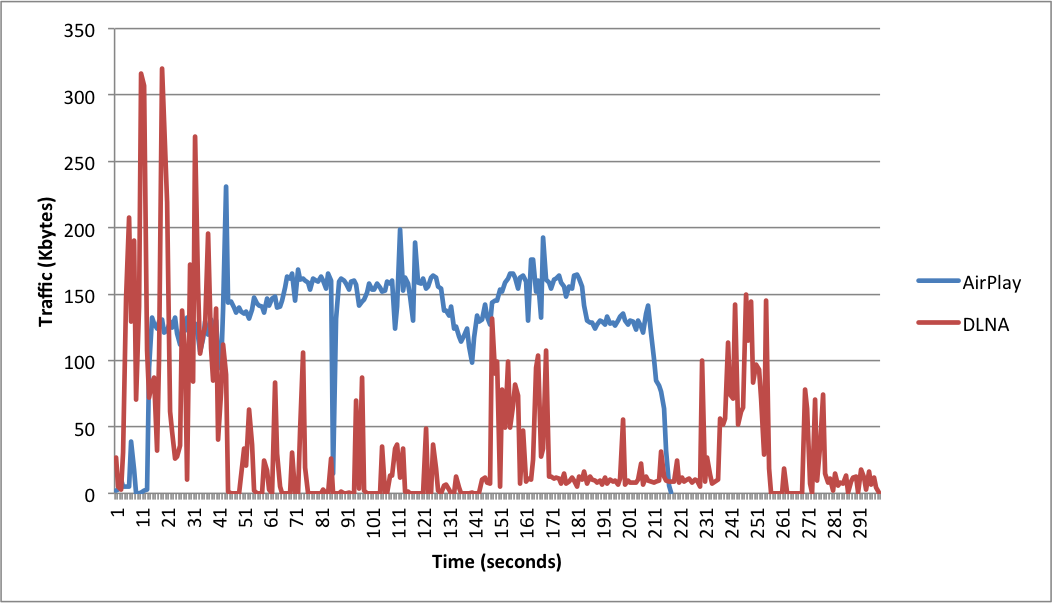
\includegraphics[width=1\columnwidth]{charts/packetloss_15percent}}
\caption{AirPlay and DLNA traffic graph in terms of packet loss
\label{all_pl_1}}
\end{figure}
\clearpage
\subsection{Statistics\label{4_2}}
16 months after its release, our application has achieved 924000 downloads from
223 countries all around the world, with a daily active user number of over
15000. Our users almost cover 99\% of all continents and a world map of our user
distribution is shown in Figure \ref{user_map}.
\begin{figure}[hb]
\centering 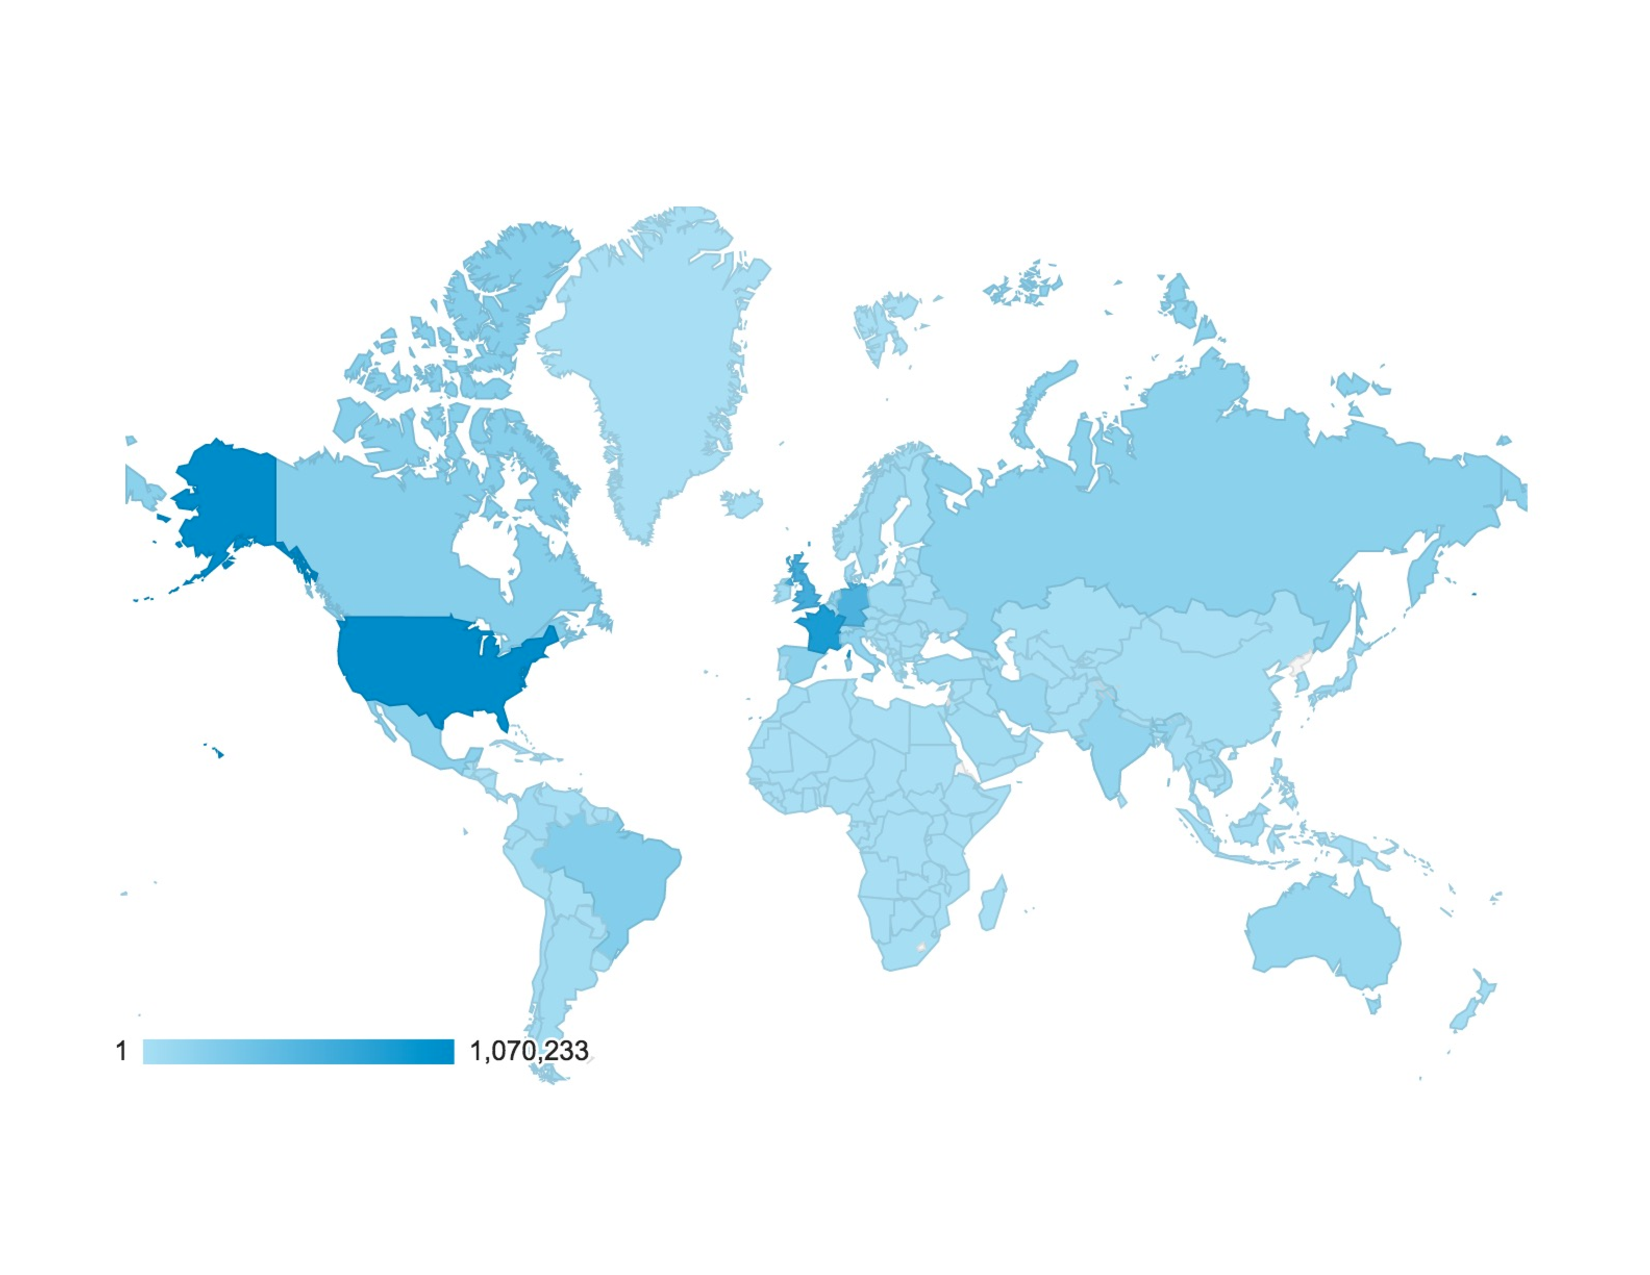
\includegraphics[width=0.9\columnwidth]{charts/session_world_map}
\caption{World map of visits \label{user_map}}
\end{figure}
So far, we have received ratings from 10253 users and currently the average
rating is 3.9 out of 5. The distribution is shown in Figure \ref{ratings}.
According to the rating distribution graph, most users are satisfied with our
solution and give the 5 stars rating. However, the average rating is heavily
influenced by the 1 star rating users. The reason for those low ratings is that
the receivers some users have in home are not compatible with our application
due to different reasons. It might be that some protocols,such as Roku box, are
not supported yet. Network condition problem also contributes to the
incompatibility issues. For example some routers have by default disabled
multicast due to security reasons. Another major cause of the incompatibility
problem is that even with the same protocol, such as DLNA, a minor
implementation difference may cause the break of connections. Thus, in the
later phase, we have made receiver specific hacks to make our application work
with most DLNA receivers, regardless of which implementation they use.
\begin{figure}[!t]
\centering 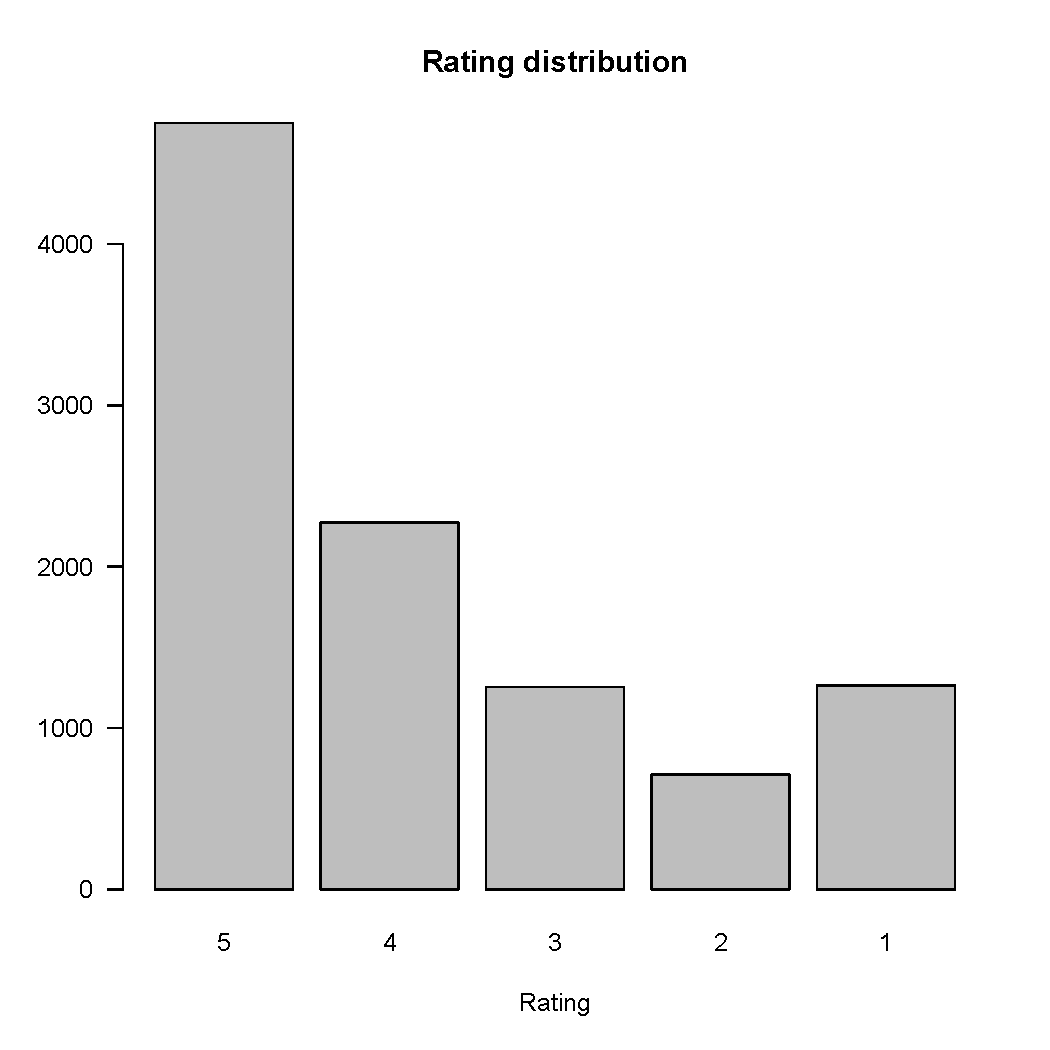
\includegraphics[height=8.5cm]{charts/rating_distribution}
\caption{Rating distribution\label{ratings}}
\end{figure}
In terms of user distribution, in the last 16 months, this application turns out
to be very popular in countries like France, United States, Germany, United Kingdom
and Brazil. The user distribution is shown in Figure \ref{user_country}.
\begin{figure}[htb]
\centering 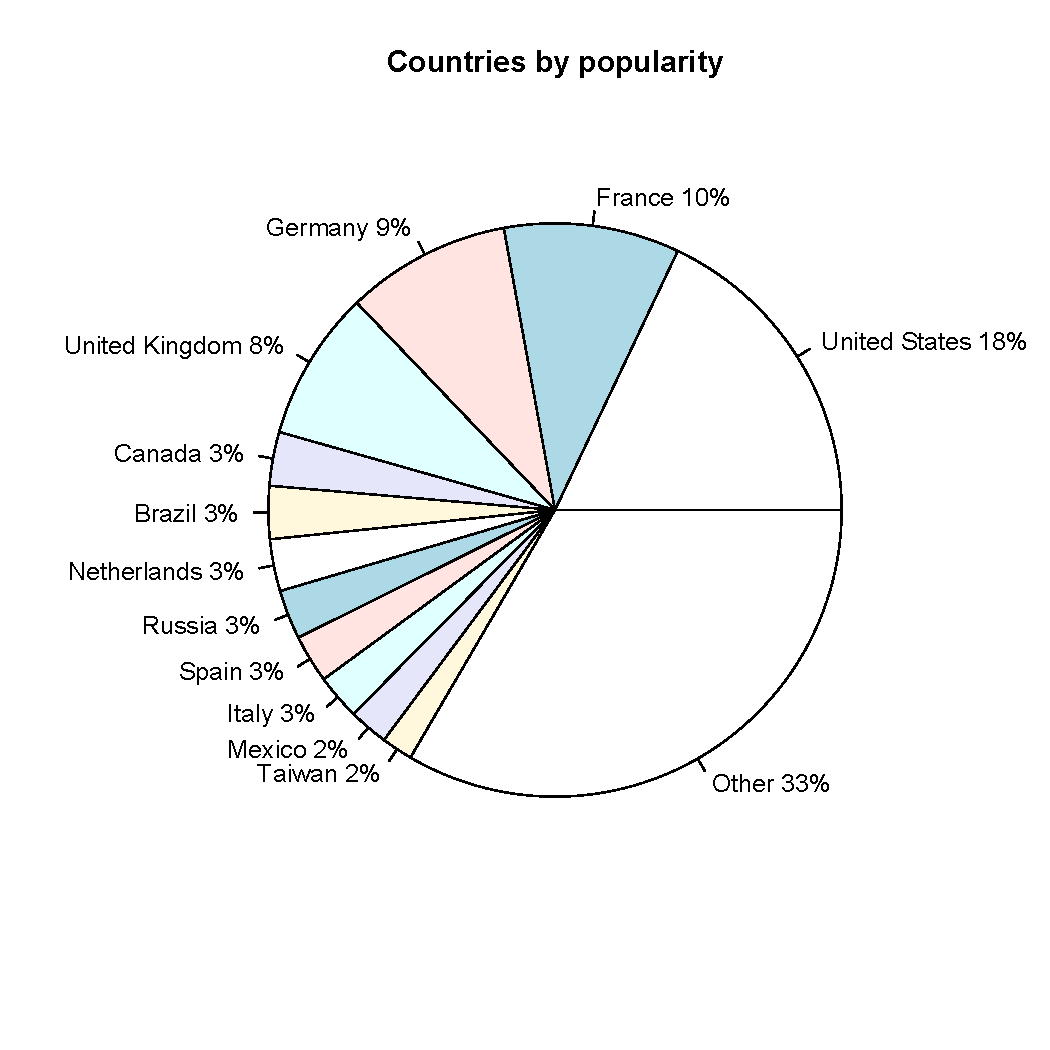
\includegraphics[height=8.5cm]{charts/country_popularity}
\caption{Popularity in different countries \label{user_country}}
\end{figure}
We have also translated the description of the application to nine languages,
which include English, Russian, German, Italian, Japanese, French, Chinese, Spanish and Korean. The multiple language support may also contribute to the popularity of our application in all parts of the world.
\begin{figure}[!t]
\centering 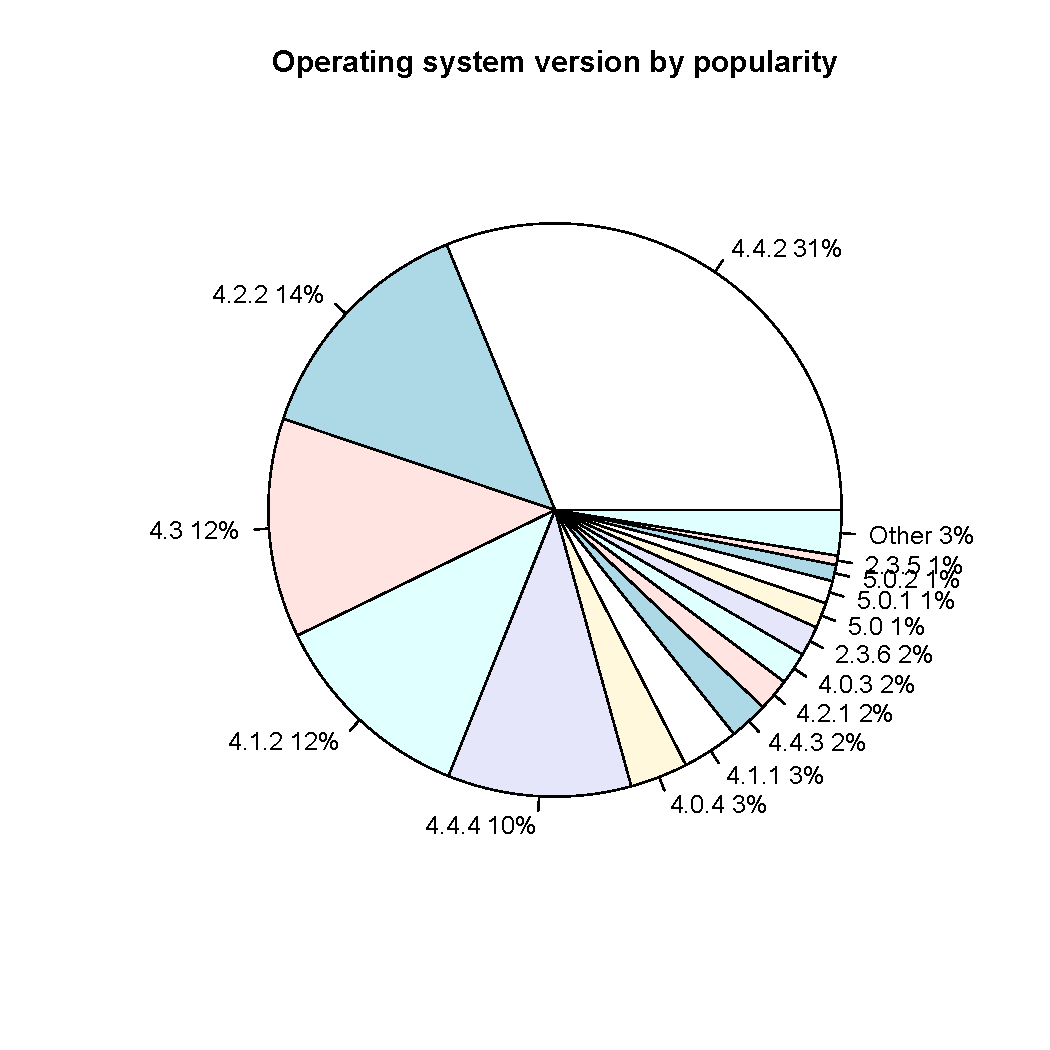
\includegraphics[height=8.5cm]{charts/os_version_popularity}
\caption{Popularity of different Android versions \label{os_versions}}
\end{figure}
The most popular operating system used for our application is Android, but
interestingly there are also tens of users using our application on
BlackBerry
\footnote{\url{https://developer.blackberry.com/playbook/android/files/webinars/BlackBerry_Runtime_for_Android_Apps.pdf}},
which is another mobile operating system developed by BlackBerry Inc.  For all
the users on the Android system, the distribution is shown in Figure
\ref{os_versions}. According to the statistics, Android Kitkart is the most
widely used Android version, which is also our target system version. Most
users have updated to the Kitkart version 4.4. We also have a very small part
of users who are using the latest Android 5.0 (Lollipop). These users are more
likely to experience more bugs. The reason is that the latest Android uses
Android RunTime (ART) to replace Dalvik runtime\cite{dalvik_arch}. The native
code (C code) support is not optimized so well for the new ART architecture.
However the native code support shall be improved in a later update of
the Android Lollipop operating system.

Since this application integrated a HTTP steaming proxy, it is possible for
other online content provider applications to use our application as the bridge
to connect to the home networking devices. Figure \ref{online_channel} shows the
the most popular online media sources used by our users. The most popular online source
is YouTube, with a total number of 115759 use times. The second popular known
proxy source is Ted with 1036 use times, followed by Viemo, which is the least popular
known online media source. Interestingly, some other third-party applications
also use our application to share their content. These third-party applications
include local file browser applications which have an embedded file server.
There are even more unknown sources that can not be distinguished by our application.
This result proves the diversity of the online content sources, and it also
demonstrates the strong interest of our end users to try our solution with
different content sources.

\begin{figure}[htb]
\centering 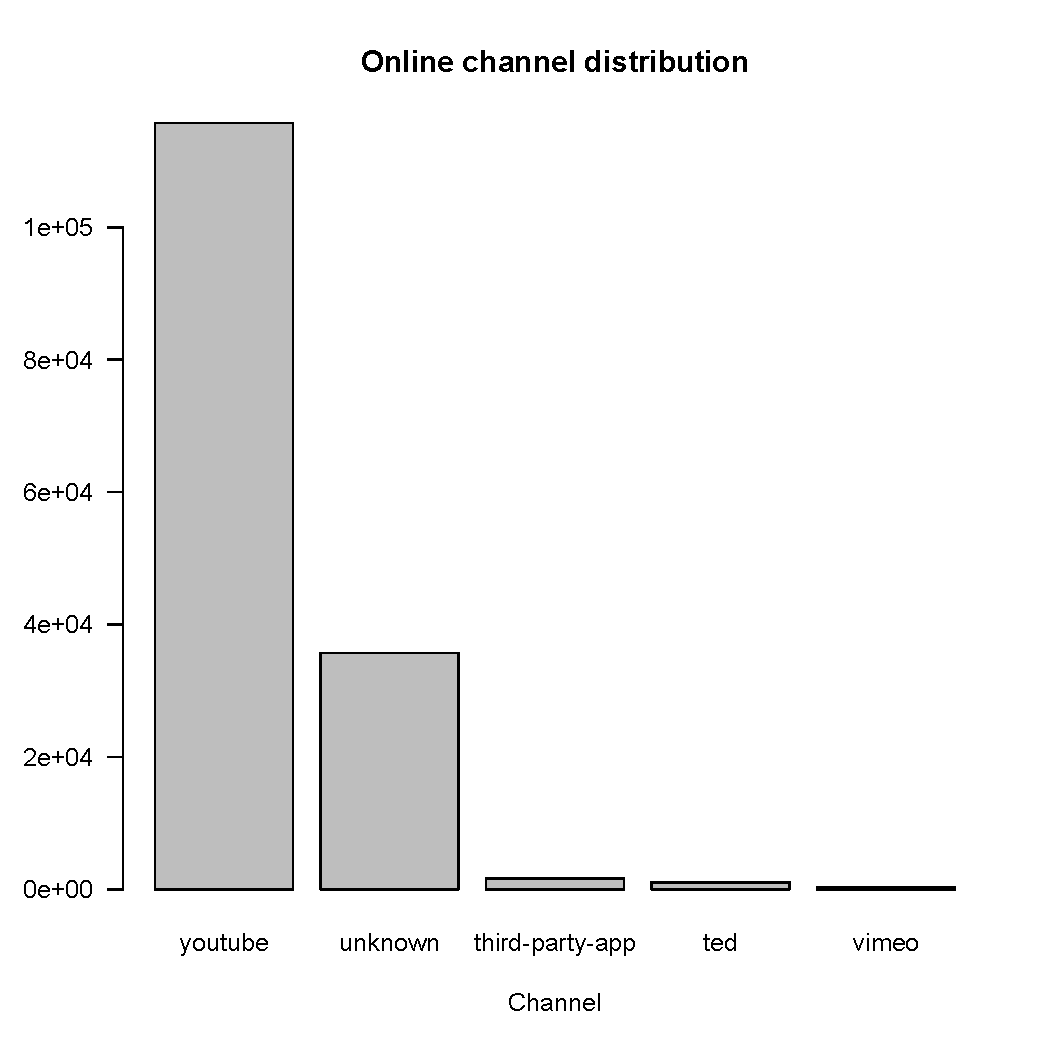
\includegraphics[height=8.5cm]{charts/online_channel}
\caption{Popularity of different online channels \label{online_channel}}
\end{figure}

The most interesting statistic of our application is the receiver popularity,
which is shown in Figure \ref{receiver_types}. Since our project aimed at
developing a solution for multimedia home networking, it is especially useful
to find out which protocol is the most popular one. According to the result
from Google Analytics, the AirPlay and DLNA are the most popular standards,
with a combined   usage rate of 87\% among all streaming sessions. Chromecast
is the third most popular receiver while Amazon Fire TV is the least adopted
receiver. The result can also suggest the future trend of multimedia home
networking.

Our application has gone public for 16 months and it has seen a series of small
updates and one major update last Christmas. The number of daily visits is
shown in Figure \ref{sessions_perday}. As shown in the figure, after the
release, the number of users has seen a great increase in the first two months.
After that, the number of active users has remained steady over the following
six months, until we launched a major release after around a year. The new
release included an updated UI and a better written streaming component. This
release has brought a significant growth in users. Currently our application is
hitting 15000 visits per day,  proving that our solution has been successful.

\begin{figure}[htb]
\centering 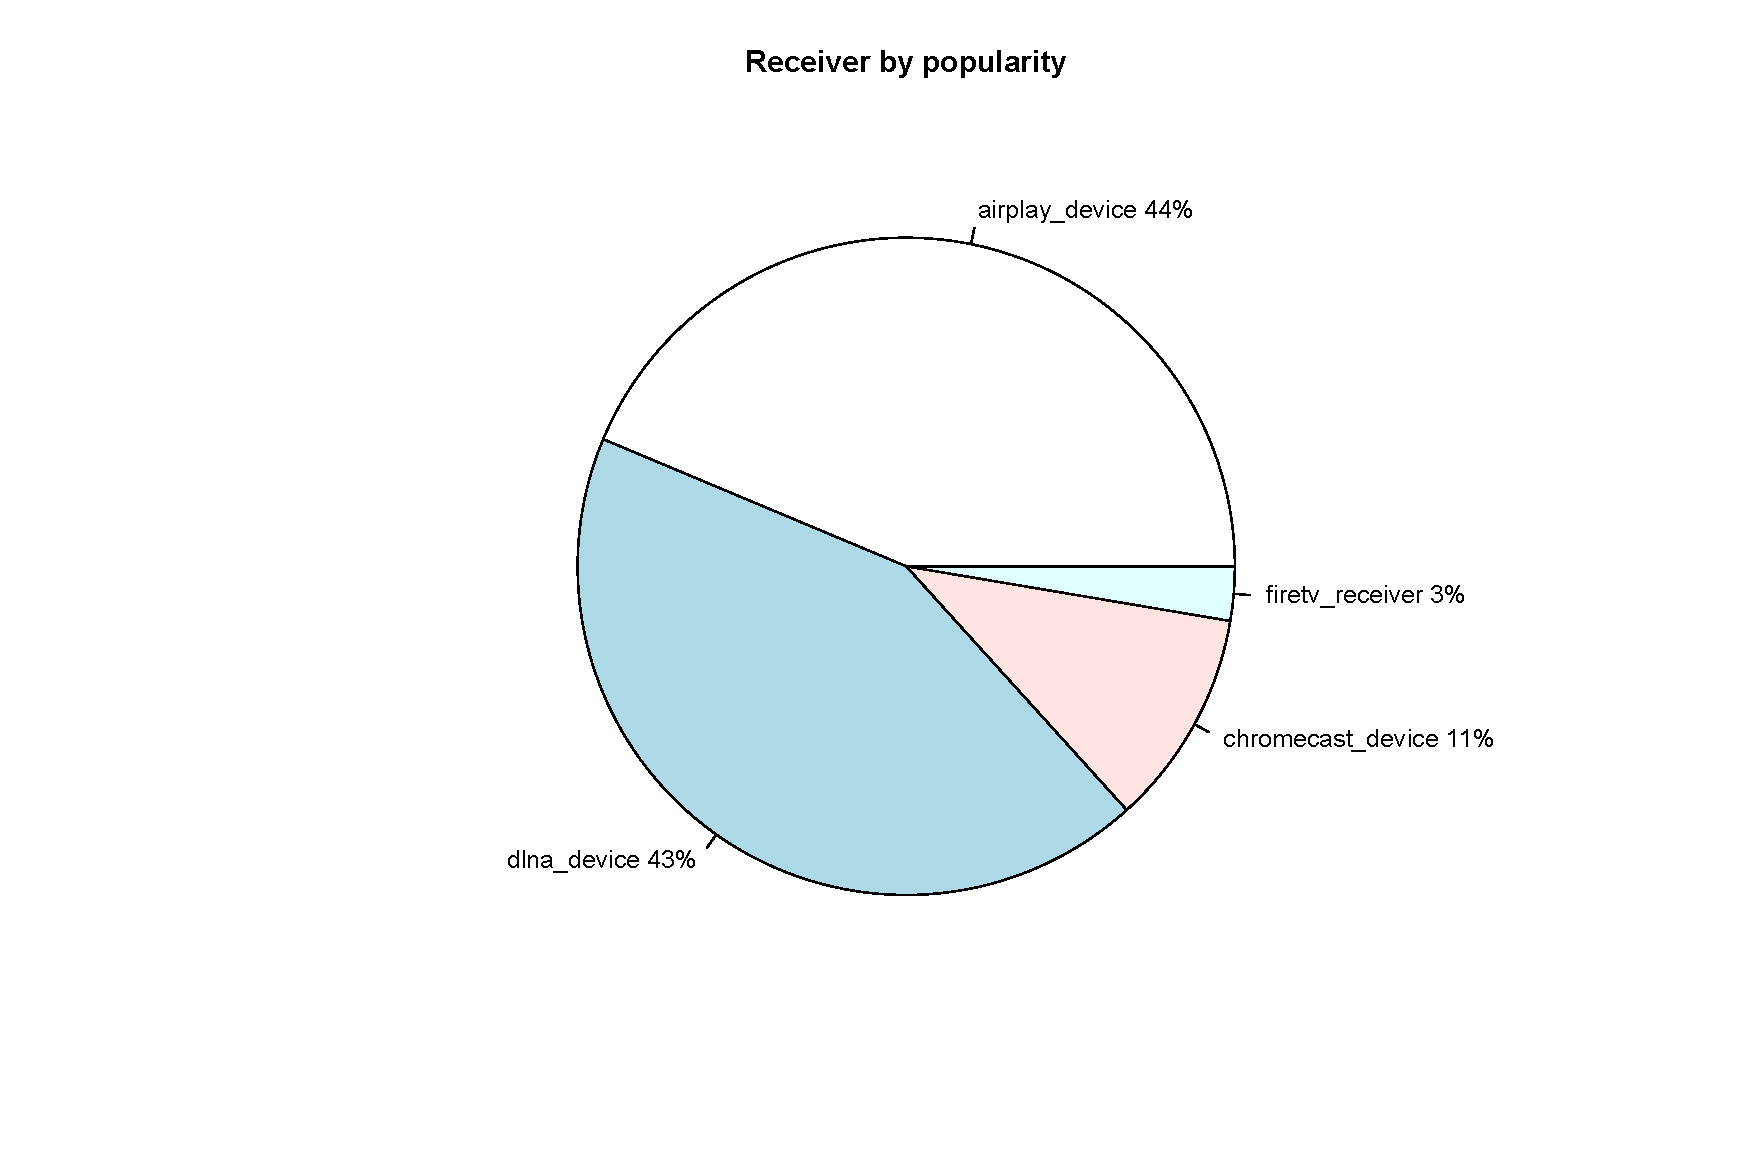
\includegraphics[height=9cm]{charts/receiver_popularity}
\caption{Popularity of receiver types \label{receiver_types}}
\end{figure}

\begin{figure}[hb]
\centering 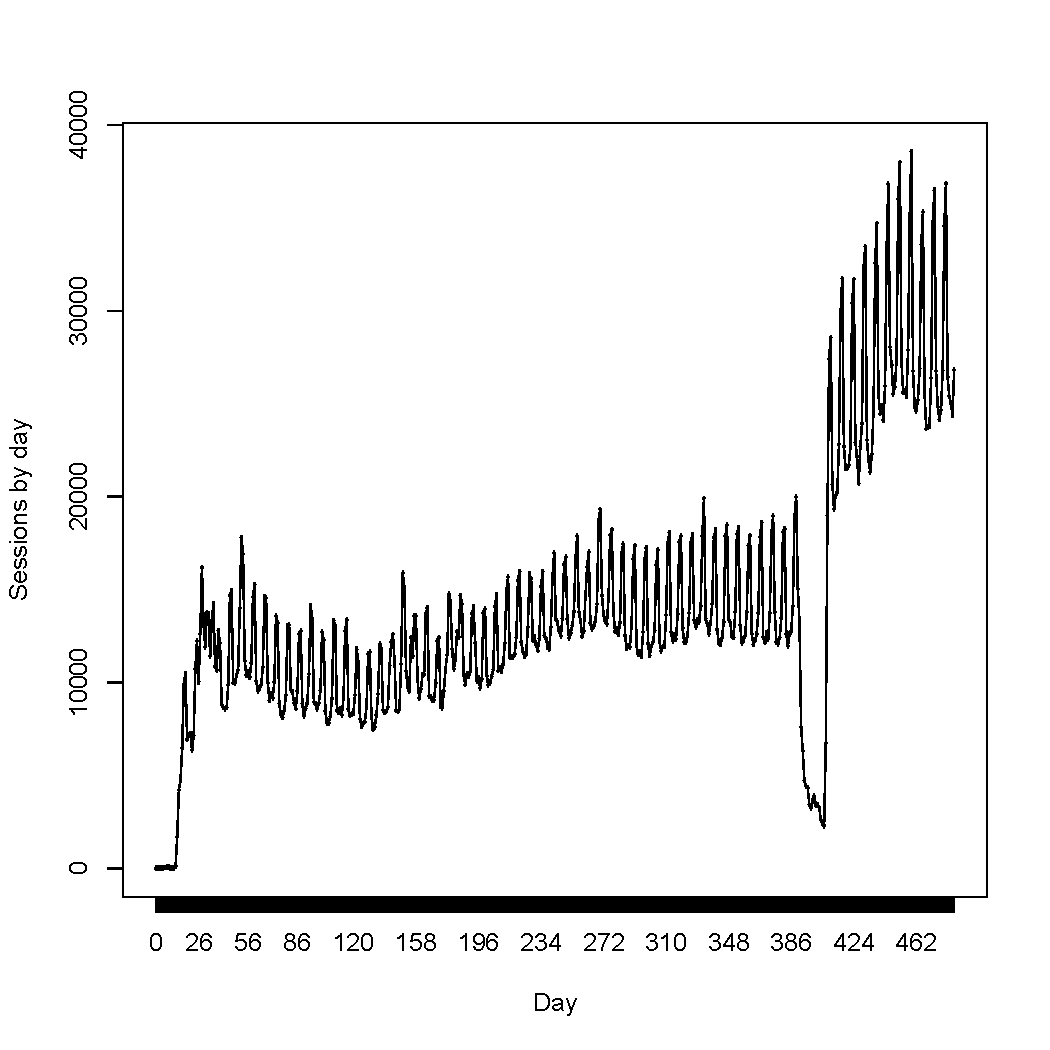
\includegraphics[height=9cm]{charts/sessions_per_day}
\caption{Sessions per day \label{sessions_perday}}
\end{figure}
\clearpage
\subsection{User study\label{4_3}}
It is essential to listen to feedback from users and our application users can
send their feedback to us in many ways, such as commenting on the Google Play
Store or sending E-mail directly to us.

Having been collecting user feedbacks for over 16 months, we have made several
improvements accordingly. Most of the feedbacks are about trouble shooting. For
example, device discovery problems has been the most common issues for most
complaining users. The reason could be that phones and other receivers are not
connected to the same Wi-Fi network, or the receivers are not turned on. With
more and more user feedback collected, we felt obliged to set up a website for
trouble shooting. After the setup of the feedback website we kept updating and
improving the trouble shooting pages. Now most complaining users could find
their answer in these trouble shooting pages.
